\documentclass[tikz]{standalone}

\usetikzlibrary{automata,positioning,calc}

\begin{document}
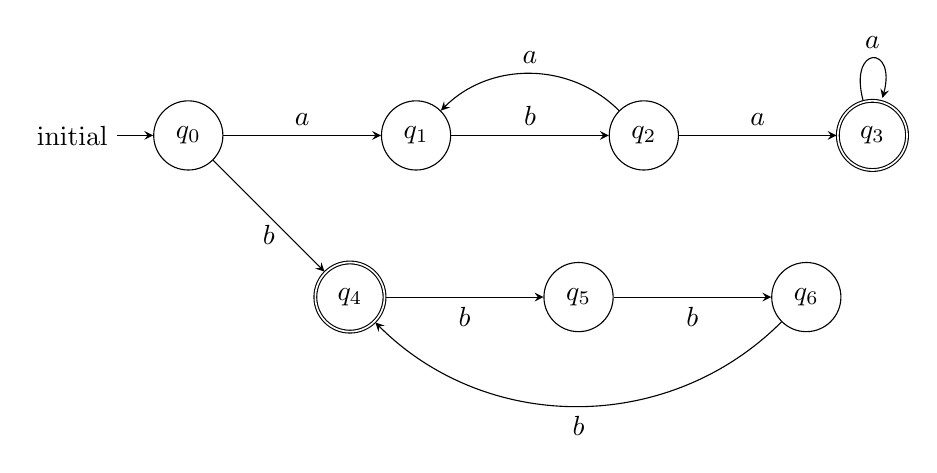
\begin{tikzpicture}[>=stealth,node distance=2,initial text={initial}]

\node [state,initial] (n0) {$q_0$};

\node [state] (n1) [right=of n0] {$q_1$};
\node [state] (n2) [right=of n1]{$q_2$};
\node [state,accepting] (n3) [right=of n2]{$q_3$};

\node [state,accepting] (n4) [below right=of n0] {$q_4$};
\node [state] (n5) [right=of n4] {$q_5$};
\node [state] (n6) [right=of n5] {$q_6$};

\path [->]
	(n0)
		edge node [above] {$a$} (n1)
		edge node [below] {$b$} (n4)
	(n1)
		edge node [above] {$b$} (n2)
	(n2)
		edge [bend right=45] node [above] {$a$} (n1)
		edge node [above] {$a$} (n3)
	(n3)
		edge [loop above] node [above] {$a$} ()
	(n4)
		edge node [below] {$b$} (n5)
	(n5)
		edge node [below] {$b$} (n6)
	(n6)
		edge [bend left=45] node [below] {$b$} (n4)
;	

\end{tikzpicture}
\end{document}
